% Choose one to switch between slides and handout
\documentclass[]{beamer}
%\documentclass[handout]{beamer}

% Video Meta Data
\title{Bitcoin, Blockchain and Cryptoassets}
\subtitle{Proof of Work}
\author{Prof. Dr. Fabian Schär}
\institute{University of Basel}

% Config File
% Packages
\usepackage[utf8]{inputenc}
\usepackage{hyperref}
\usepackage{gitinfo2}
\usepackage{tikz}
\usepackage{amsmath}
\usepackage{mathtools}
\usepackage{bibentry}
\usepackage{xcolor}
\usepackage{colortbl} % Add colour to LaTeX tables
\usepackage{caption}
\usepackage[export]{adjustbox}
\usepackage{pgfplots} \pgfplotsset{compat = 1.17}
\usepackage{makecell}
\usepackage{fancybox}
\usepackage{ragged2e}
\usepackage{fontawesome}
\usepackage{seqsplit}
\usepackage{tabularx}

% Color Options
\definecolor{highlight}{rgb}{0.65,0.84,0.82}
\definecolor{focus}{rgb}{0.72, 0, 0}
\definecolor{lightred}{rgb}{0.8,0.5,0.5}
\definecolor{midgray}{RGB}{190,195,200}

% Beamer Template Options
\beamertemplatenavigationsymbolsempty
\setbeamertemplate{footline}[frame number]
\setbeamercolor{structure}{fg=black}
\setbeamercolor{footline}{fg=black}
\setbeamercolor{title}{fg=black}
\setbeamercolor{frametitle}{fg=black}
\setbeamercolor{item}{fg=black}
\setbeamercolor{}{fg=black}
\setbeamercolor{bibliography item}{fg=black}
\setbeamercolor*{bibliography entry title}{fg=black}
\setbeamercolor{alerted text}{fg=focus}
\setbeamertemplate{items}[square]
\setbeamertemplate{enumerate items}[default]
\captionsetup[figure]{labelfont={color=black},font={color=black}}
\captionsetup[table]{labelfont={color=black},font={color=black}}

\setbeamertemplate{bibliography item}{\insertbiblabel}

% Link Icon Command
\newcommand{\link}{%
    \tikz[x=1.2ex, y=1.2ex, baseline=-0.05ex]{%
        \begin{scope}[x=1ex, y=1ex]
            \clip (-0.1,-0.1)
                --++ (-0, 1.2)
                --++ (0.6, 0)
                --++ (0, -0.6)
                --++ (0.6, 0)
                --++ (0, -1);
            \path[draw,
                line width = 0.5,
                rounded corners=0.5]
                (0,0) rectangle (1,1);
        \end{scope}
        \path[draw, line width = 0.5] (0.5, 0.5)
            -- (1, 1);
        \path[draw, line width = 0.5] (0.6, 1)
            -- (1, 1) -- (1, 0.6);
        }
    }

% Read Git Data from Github Actions Workflow
% Defaults to gitinfo2 for local builds
\IfFileExists{gitInfo.txt}
	{\input{gitInfo.txt}}
	{
		\newcommand{\gitRelease}{(Local Release)}
		\newcommand{\gitSHA}{\gitHash}
		\newcommand{\gitDate}{\gitAuthorIsoDate}
	}

% Custom Titlepage
\defbeamertemplate*{title page}{customized}[1][]
{
  \vspace{-0cm}\hfill\includegraphics[width=2.5cm]{../config/logo_cif}
  \includegraphics[width=1.9cm]{../config/seal_wwz}
  \\ \vspace{2em}
  \usebeamerfont{title}\textbf{\inserttitle}\par
  \usebeamerfont{title}\usebeamercolor[fg]{title}\insertsubtitle\par  \vspace{1.5em}
  \small\usebeamerfont{author}\insertauthor\par
  \usebeamerfont{author}\insertinstitute\par \vspace{2em}
  \usebeamercolor[fg]{titlegraphic}\inserttitlegraphic
    \tiny \noindent \texttt{Release Ver.: \gitRelease}\\ 
    \texttt{Version Hash: \gitSHA}\\
    \texttt{Version Date: \gitDate}\\ \vspace{1em}
    
    
    \iffalse
  \link \href{https://github.com/cifunibas/Bitcoin-Blockchain-Cryptoassets/blob/main/slides/intro.pdf}
  {Get most recent version}\\
  \link \href{https://github.com/cifunibas/Bitcoin-Blockchain-Cryptoassets/blob/main/slides/intro.pdf}
  {Watch video lecture}\\ 
  
  \fi
  
  \vspace{1em}
  License: \texttt{Creative Commons Attribution-NonCommercial-ShareAlike 4.0 International}\\\vspace{2em}
  \includegraphics[width = 1.2cm]{../config/license}
}


% tikzlibraries
\usetikzlibrary{decorations.pathreplacing}
\usetikzlibrary{decorations.markings}
\usetikzlibrary{positioning}
\usetikzlibrary{calc}
\captionsetup{font=footnotesize}


%%%%%%%%%%%%%%%%%%%%%%%%%%%%%%%%%%%%%%%%%%%%%%
%%%%%%%%%%%%%%%%%%%%%%%%%%%%%%%%%%%%%%%%%%%%%%
\begin{document}

\thispagestyle{empty}
\begin{frame}[noframenumbering]
	\titlepage
\end{frame}

%%%
\begin{frame}{Competition via Resource Allocation}

Basic Idea: An activity that can be executed too quickly is \color{focus}combined with a probabilistic trial and error task\color{black}. The activity can only be executed if the task is solved correctly.

\uncover<2->{
	\vspace{1.5 em}

	$\Rightarrow$ Only a small fraction of tries will lead to the desired result. 
}
\end{frame}
%%%	

%%%
\begin{frame}{Origins of Proof of Work}
	
	The concept of Proof of Work was proposed in 1993 \cite{dwork_pricing_1993} to help deter spam and denial of service attacks. 
	
	\vspace{1.5em}
	
	Other mechanisms have been popularized in the meantime, but Proof of Work remains the best known mechanism to deter sybil attacks and still sees widespread usage due to its simplicity.

\end{frame}
%%%	

%%%
\begin{frame}{In the Context of Bitcoin}

Proof of Work in the context of Bitcoin solves the following problems:

\begin{itemize}
	\item Blocks need to be created within certain time intervals
	\begin{itemize}
		\item Not too fast (Propagation delay)
		\item Not too slow (Transaction throughput)
	\end{itemize}
	\item The chain must be protected from simple replication
	\item Malicious behavior when creating blocks should be discouraged 
\end{itemize}

\end{frame}
%%%

%%%
\begin{frame}{Implementation in the Bitcoin Protocol}

In the Bitcoin protocol, Proof of Work is implemented in the context of \color{focus}block header hash values\color{black}. The properties of the \texttt{dSHA256} hash function make it impossible to create a block header hash with a desired value.

\uncover<2->{
	\vspace{1.5em}
	\textbf{Trial and Error:}
	\begin{itemize}
		\item Require certain properties from valid block header hashes
		\item Specifically: Below a certain threshold value
		\item Each newly created block candidate has a random chance to satisfy the criteria
	\end{itemize}
}

\uncover<3->{
	\vspace{0.5em}
	$\Rightarrow$ Create new block candidates until the block header hash value is sufficiently low
}
 	
\end{frame}
%%%	

%%%
\begin{frame}{A Simple Example}
	Assume the current threshold values is
	\seqsplit{0x1000000000000000000000000000000000000000000000000000000000000000}.
	
	\begin{itemize}
		\item To be lower than this value, a hash must contain a 0 in the first position
		\item When generating a hash from a given input, each digit has a 1 in 16 chance to be of a certain value
	\end{itemize}

	\uncover<2->{
		\vspace{0.5em}
		$\Rightarrow$ The network would need to generate an average of 16 candidate blocks before being able to extend the chain.
	}
	
\end{frame}
%%%	

%%%
\begin{frame}{Mining Bitcoin}
	The iterative process of creating block candidates and checking their block header hash values against the threshold is called \color{focus}mining\color{black}.
	
	
	\uncover<2->{
		\vspace{1.5em}
		Block header hash value $\geq$ threshold
		\begin{itemize}
			\item Discard the candidate block
			\item Change the contents of the block header
			\item Recompute the new block header hash value
		\end{itemize}	
	}

	\uncover<3->{
		\vspace{.5em}
		Block header hash value $<$ threshold
		\begin{itemize}
			\item The candidate block is relayed to the network
			\item The block can be appended to the chain
		\end{itemize}	
	}
	
\end{frame}
%%%	

%%%
\begin{frame}{Mining Process Model}
	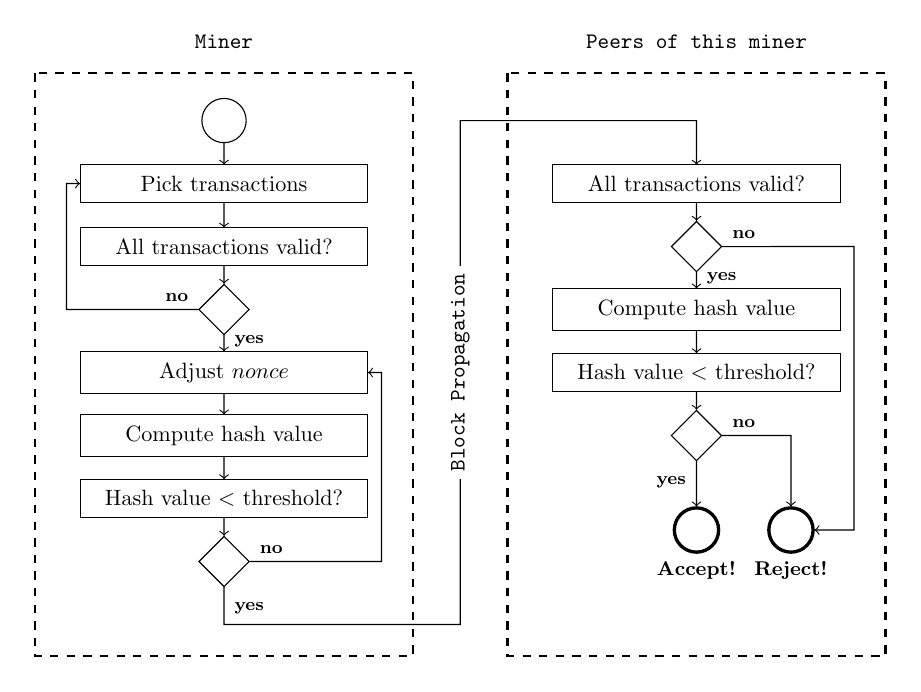
\begin{tikzpicture}[scale=0.8, every node/.style={scale=0.8}]
		\node (a) at (-3,1.25) {};
\node (b) at (3,-8) {};
\draw[dashed, thick] (a) rectangle (b);
\node at (0,1.75) {\texttt{Miner}};

\node (c) at (4.5,1.25) {};
\node (d) at (10.5,-8) {};
\draw[dashed, thick] (c) rectangle (d);
\node at (7.5,1.75) {\texttt{Peers of this miner}};

\node [draw, outer sep=0,inner sep=5,minimum width=130] (v1) at (0,-0.5) {Pick transactions};
\node [draw,outer sep=0,inner sep=5,minimum width=130] (v2) at (0,-1.5) {All transactions valid?};
\node [draw, shape=circle, minimum size=20] (v3) at (0,0.5) {};
\node [draw, minimum size=16, rotate=45] (v4) at (0,-2.5) {};


\draw [->] (v3) edge (v1);
\draw [->] (v1) edge (v2);
\draw [->] (v2) edge (v4);
\draw [->](v4) -- (-2.5,-2.5) -- (-2.5,-0.5) -- (v1) ;
\node [draw,outer sep=0,inner sep=5,minimum width=130] (v5) at (0,-3.5) {Adjust $nonce$};
\node [draw,outer sep=0,inner sep=5,minimum width=130] (v6) at (0,-4.5) {Compute hash value};
\node [draw,outer sep=0,inner sep=5,minimum width=130] (v7) at (0,-5.5) {Hash value $<$ threshold?};
\draw [->] (v4) edge (v5);
\draw [->] (v5) edge (v6);
\draw [->] (v6) edge (v7);
\node [draw, minimum size=16, rotate=45] (v8) at (0,-6.5) {};
\draw [->] (v7) edge (v8);
\draw [->](v8) -- (2.5,-6.5) -- (2.5,-3.5) -- (v5);
\node [draw,outer sep=0,inner sep=5,minimum width=130] (v9) at (7.5,-0.5) {All transactions valid?};
\node[rotate=90] (bp) at (3.75,-3.5) {\texttt{Block Propagation}};
\draw [-](v8) -- (0,-7.5) -- (3.75,-7.5) -- (bp);
\draw[->](bp) -- (3.75, 0.5) -- (7.5,0.5) -- (v9);

\node[above] at (-0.75,-2.5) {\footnotesize\textbf{no}};
\node at (0.4,-3) {\footnotesize\textbf{yes}};

\node[above] at (0.75,-6.5) {\footnotesize\textbf{no}};
\node at (0.4,-7.25) {\footnotesize\textbf{yes}};

\node [draw, minimum size=16, rotate=45] (v10) at (7.5,-1.5) {};
\node [draw,outer sep=0,inner sep=5,minimum width=130] (v14) at (7.5,-2.5) {Compute hash value};
\node [draw,outer sep=0,inner sep=5,minimum width=130] (v15) at (7.5,-3.5) {Hash value $<$ threshold?};
\node [draw, minimum size=16, rotate=45] (v11) at (7.5,-4.5) {};

\node [draw, very thick, shape=circle, minimum size=20, label=below:\small\textbf{Accept!}] (v12) at (7.5,-6) {};
\node [draw, very thick, shape=circle, minimum size=20, label=below:\small\textbf{Reject!}] (v13) at (9,-6) {};

\draw [->] (v9) edge (v10);
\draw [->] (v10) edge (v14);
\draw [->] (v14) edge (v15);
\draw [->] (v15) edge (v11);
\draw [->] (v11) edge (v12);
\draw [->](v11) -- (9,-4.5) -- (v13);
\draw [->](v10) -- (10,-1.5) -- (10,-6) -- (v13);

\node[above] at (8.25,-1.5) {\footnotesize\textbf{no}};
\node at (7.9,-2) {\footnotesize\textbf{yes}};
\node[above] at (8.25,-4.5) {\footnotesize\textbf{no}};
\node at (7.1,-5.25) {\footnotesize\textbf{yes}};
	\end{tikzpicture}
\end{frame}
%%%	

%%%
\begin{frame}{Dynamic Threshold}
	The threshold parameter $\delta$ is dynamically adjusted so that the network will produce a valid block on average every ten minutes.
	
	\uncover<2->{
		\vspace{1.5em}
		\begin{itemize}
			\item The adjustment happens every 2'016 valid blocks
			\item Assuming 10 minute blocks, this is every 14 days
			\item The new threshold value $\delta$ is calculated based on the expected value $E(t)$ and the actual duration $t$
		\end{itemize}
	}

	\uncover<3->{
		\begin{center}
		\begin{align*}
			\delta_{new} &= \delta_{old} \cdot \frac{t}{E(t)} \\
			             &= \delta_{old} \cdot \frac{t}{2016 \cdot 10}
		\end{align*}
		\end{center}

	}
\end{frame}
%%%	

%%%
\begin{frame}{Dynamic Threshold}
	Blocks are generated faster than expected $t < E(t)$:
	\begin{itemize}
		\item $\frac{t}{E(t)}$ will be between 0 and 1 $\Rightarrow \delta_{new} < \delta_{old}$
		\item A lower threshold value will lead to fewer accepted block candidates in the following period
	\end{itemize}

	\uncover<2->{
		\vspace{1.5em}
		Blocks are generated slower than expected $t > E(t)$:
		\begin{itemize}
			\item $\frac{t}{E(t)}$ will be above 1 $\Rightarrow \delta_{new} > \delta_{old}$
			\item A higher threshold value will lead to more accepted block candidates in the following period
		\end{itemize}
	}

	\uncover<3->{
		\vspace{1.5em}
		In both cases the average block creation time is moved closer to 10 minutes again.
	}
\end{frame}
%%%	

%%%
\begin{frame}{Difficulty}
	\begin{figure}[t]
		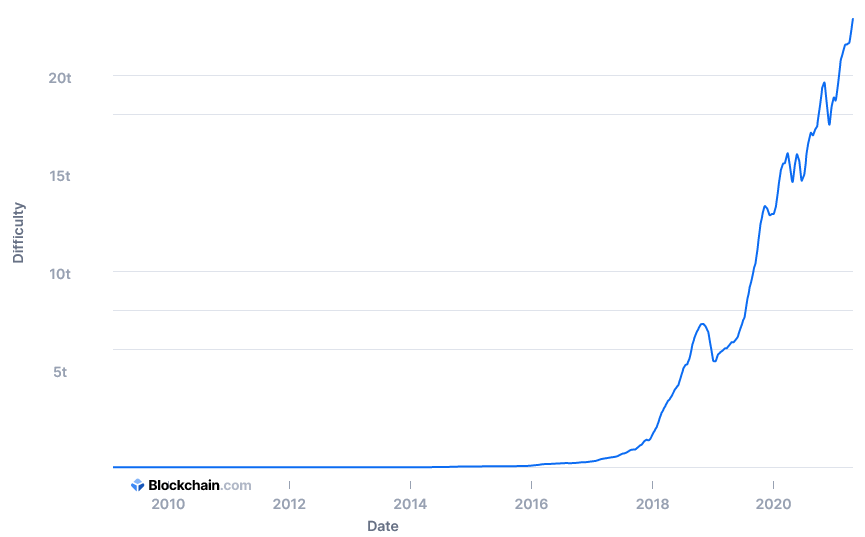
\includegraphics[height=\textheight/2]{../assets/images/difficulty}
		
		\tiny Source: \link \url{https://www.blockchain.com/charts/difficulty}, April 2021
	\end{figure}
	
	
	
	The Difficulty $D$ shows the change of the threshold parameter over time. It is equal to the maximum threshold $\delta(B_0)$ divided by the current threshold $\delta(B_i)$.
	\begin{center}
		$D_i \coloneqq \frac{\delta(B_0)}{\delta(B_i)}$
	\end{center}
\end{frame}
%%%	

%%%
\begin{frame}{Incentives}
Miners face costs. They must be incentivized:

\begin{enumerate}
	\item Newly minted Bitcoin units (UTXO with no inputs)
	\item Transaction fees (Difference between inputs and outputs of all trx in block)
\end{enumerate} \vspace{1em}

\uncover<2->{
Every 210,000 blocks (approx. 4 yrs), the reward rate is halved. Initially, it was at 50 Bitcoin per block.
\vspace{-2em}
\center
	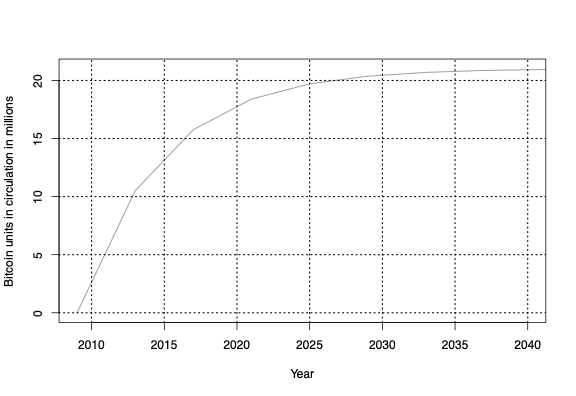
\includegraphics[width=9cm]{../assets/images/bitcoin_growth.png}
	}
\end{frame}
%%%

\begin{frame}%[allowframebreaks]
	\frametitle{References}
	\bibliographystyle{amsplain}
	\bibliography{../assets/bib/refs}
\end{frame}

\end{document}